%% $Id$

%% Copyright (c)  1998-2010
%% by  RWTH-Aachen, Germany
%% Some rights reserved.

%% This work is licensed under the Creative Commons Attribution-Share
%% Alike 3.0 License. To view a copy of this license, visit
%% http://creativecommons.org/licenses/by-sa/3.0/ or send a letter to
%% Creative Commons, 171 Second Street, Suite 300, San Francisco,
%% California, 94105, USA.

\section{Development Policies}

This chapter outlines the policy decisions that were made for the ViSTA development process.
It cares about the different versions and revisions, and the way in which changes have to be worked in and tested.

\subsection{Nomenclature}
It is important to define some basic vocabulary in order to know what this document is talking about.

\begin{itemize}

\item \textbf{\code{ViSTA} core libraries}. The \code{ViSTA} core libraries are defined as the set of the following libraries. See Figure~\ref{fig:ViSTAArchitecture} for the basic layout of the \code{VISTA} core libraries.
  \begin{itemize}
  \item \code{VistaBase}. 
    This library provides basic constructs such as guaranteed-size typedefs, vector math types, general tools for timing, streams, and exceptions.
  \item \code{VistaAspects}. 
    This library represents a collection of abstract interfaces for usage by other libraries.
  \item \code{VistaInterProcComm} (IPC).
  	Classes and strategies for Inter-process communication, e.g., networking and concurrency synchronizations.
  \item \code{VistaTools}.
  	A collection of often to use tools and algorithms, e.g., file handling, octree data structures and protocols.
  \item \code{VistaMath}.
  	Comfortable, but maybe slow, interfaces and mathematical algorithms.
  \item \code{VistaDeviceDrivers}.
  	Low-Latency framework for input device handling. Drivers and driver plugins for VR interaction devices (trackers, gamepads, HID devices, MIDI, WiiMote...)
  \item \code{DataFlowNet}.
  	Dataflow-based framework for input data transformation and processing.
  \item \code{VistaKernel}.
  	Basic VR Toolkit functionality, i.e. displays and interaction devices, scenegraph API, standard behaviors and event management.
  \item \code{VistaKernelOpenSGExt}.
  	Contains extended functionality based on the OpenSG implementation.
  \end{itemize}

\item \textbf{\code{ViSTA} add-on libraries}.
  Libraries that realize functionality on top of the \code{ViSTA} core libraries, e.g., the \code{ViSTAMedia, VRZula, VistaCollisionDetection}.

\item \textbf{3rd party libraries}.
  Additional software packages that are not developed as part of this project, e.g., OpenSG, FOX or libXML.

\item \textbf{\code{ViSTA} applications}.
  VR applications that are realized at least on the \code{ViSTA} core libraries and may depend on other 3rd party or \code{ViSTA} libraries.

\end{itemize}

\begin{figure}
\begin{center}
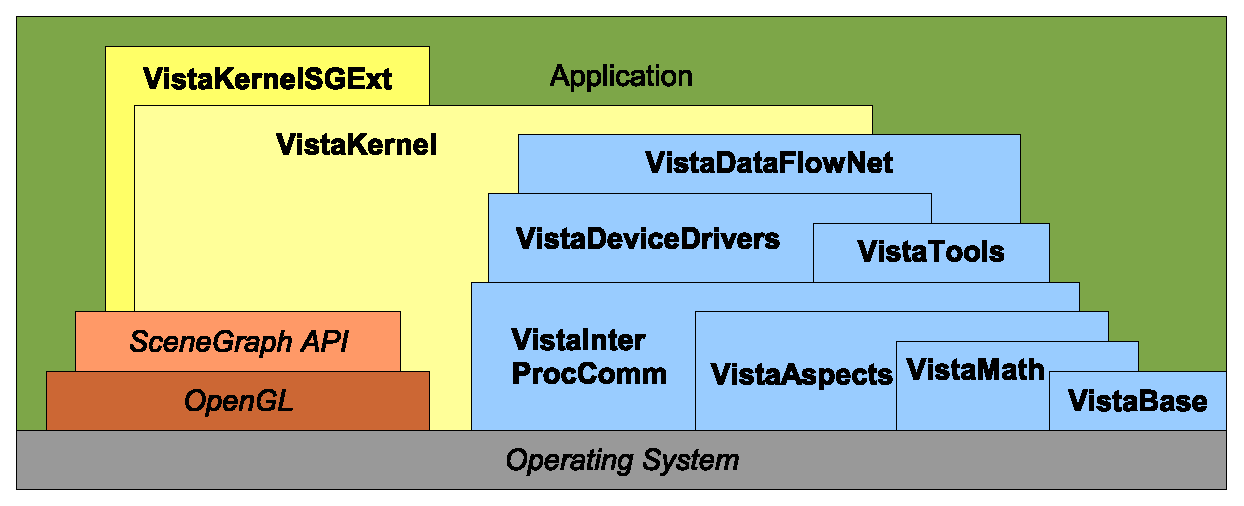
\includegraphics[width=10cm]{ViSTAArchitecture}
\end{center}
\caption{\label{fig:ViSTAArchitecture}
  The \code{ViSTA} core library principle architecture for a VR application which relies on the \code{ViSTA} core libraries only.
  Note that it is still possible to access the VistaTools, VistaAspects, VistaInterProcComm, VistaDeviceDrivers, DataFlowNet and VistaMath, although the sketch here suggests that these layers are not acessable and hidden by the VistaKernel.}
\end{figure}
 
\subsection{Roles}
The development process we discuss here differentiates between different roles.

The \textit{project maintainer} is the person that is responsible for overall library development decisions.
This means the maintainer has the last word regarding questions like
\begin{itemize}
\item when/how releases are done
\item wether to include a certain feature or not
\item which external dependencies are allowed
\item how the overall library development will progress
\end{itemize}
He is the first person to ask for general (strategic) questions regarding the library development.
The current \code{ViSTA} maintainer is Dominik Rausch (rausch@vr.rwth-aachen.de).

The \textit{developer} is supposed to work on the project, but should not decide about the external versioning (e.g., tagging) of the developed product or the used libraries.

\subsection{Library Development}
Overall development of the \code{ViSTA} core libraries should be done according to the rules described in this section.
In addition, regulations regarding coding style can be found in chapter \ref{coding_styles}.

\subsubsection{Subversion Repository policies}
At the moment, the \code{ViSTA} source code is hosted in a subversion repository SourceForge.net.
The repository is organized on the topmost level like most SVN repos, containing the top-level directories
\begin{itemize}
\item\code{branches/}
\item\code{tags/}
\item\code{trunk/}
\end{itemize}
with their usual meaning.

In general, development of new features happens in \code{trunk}.
The \code{branches} directory contains a directory for each \code{ViSTA} release as well as for optional development branches. 
For details on the release and branching strategy, see the section \ref{vista_releases} below.
In the \code{tags} folder, snapshots of the library at a certain point in time are taken.
The content of subfolders in \code{tags} should never be changed again according to the definition of a tag, although SVN allows this.
Exceptions to this should be well justified and the maintainer should be consulted beforehand.

All regular development of the library is supposed to happen in \code{trunk}.
However, we strive for a \code{trunk} which compiles at all times and is not in an unusable state, meaning that bigger parts of the library don't work at all, e.g. because of bigger conceptual changes.

Threrefore, if there are big API or conceptual changes which impact other code, where the author knows that either:

\begin{itemize}
\item he won't be able to adapt all code which is influenced by his changes and verify that the changes break no other functionality
\item he is designing a new/experimental API which is likely to still change substantially
\item he wants to commit changes or a new implementation, but is unable to test the code on all supported platforms
\end{itemize}

then the code should be commited to a development branch first, until the API stabilizes and has been tested on all supported platforms.
The functionality should of course be merged back into the main development line as soon as possible.
Mergind the changes back to the \code{trunk} is the responsibility of the developer who created the branch, and should happen in accordance with the \code{ViSTA} maintainer.

\minisec{Commit logs}
Commit messages must be in english.
We consider the usage of the following hints to what has been done to a module as given in the following table.

\begin{tabular}{|l|p{12cm}|}\hline
APIADD   & added some methods or other public symbols (typedefs, nested types, ...) to the signature of a class.\\\hline
APICHG   & changed the signature of a class.\\\hline
APIREM   & removed methods or other symbols from the signature of a class.\\\hline
ADD      & added something (e.g., resources, new module files).\\\hline
CHG      & changed something that was already there.
           This could e.g.\ be a change in a method's behavior or a better implementation.\\\hline
REM      & removed something, (e.g.\ complete modules, resources or functionality).\\\hline
FIX      & fixed an implementation in a code file.
           Try to roughly describe what was fixed.\\\hline
STYLE    & issues dealing with changes due to style guides or personal preference without implact in the functional behavior or the syntax.\\\hline
\end{tabular}

Try to point out a reference to each line in the commit log where your change was applied to.
This means that you might be checking in more than just one file, and it is not always clear to what exactly you refer in the commit log.

As an example, the following commit log is given.
\begin{verbatim}
From: VistaAspects/VistaPropertyAwareable.cpp

APIADD: added API to set a hint for PROPT_LIST 
        list member types
APICHG: added extra parameter to respect that 
        flag in PropertyList private API
CHG:    serializing the list sub type for PropertyLists now
APICHG: added extra template (default) argument to 
        specify property type for reflectionable getters 
        and setters in reflectionable code, 
        should be backwards compatible
STYLE:  removed some trailing ","
\end{verbatim}

As you can see from this example, it might not always be clear what you actually did to the module, unless you are a developer of that module yourself.
Think of this when writing commit log messages.
As an additional value, using the differential to the previous version give additional hints on what has acually been done to the module.


\subsubsection{External libraries and packages}
Every software code resource which is used and not developed as part of the \code{ViSTA} project is called \emph{external} or \emph{3rd party} software.

\minisec{Legal issues}
For all \code{ViSTA} development it is absolutely mandatory to respect the legal constraints that 3rd party software is shipped with.
In general, for ViSTA libraries, only software code that complies with the current license regulations of \code{ViSTA} itself is to be used.
As the current \code{ViSTA} version is released under LGPLv3, only licenses which the FSF considers compatible with the LGPL are permitted.
If in doubt, visit the page \texttt{http://www.gnu.org/licenses/license-list.html\#GPLCompatibleLicenses}. 
In any case you should contact the \code{ViSTA} maintainer before deciding on any new 3rd party software to be used in \code{ViSTA}.

\subsection{Release guidelines}

\subsubsection{\code{ViSTA} versioning}
Each \code{ViSTA} release has a version number of the form \code{X.Y.Z}, where
\begin{itemize}
\item\code{X} is called the ``major version'',
\item\code{Y} is called the ``minor version'',
\item\code{Z} is called the ``revision''.
\end{itemize}

To make the different versions distinguishable by user code, \code{VistaKernel/VistaVersion.h} must contain the following preprocessor defines
\begin{itemize}
\item\code{VISTA\_RELEASE\_NAME}
\item\code{VISTA\_VERSION}
\item\code{VISTA\_MAJOR}
\item\code{VISTA\_MINOR}
\item\code{VISTA\_REVISION}
\end{itemize}



\subsubsection{\code{ViSTA} releases}
\label{vista_releases}
If the current trunk is considered stable enough and it is time for a release, we branch off with a new release branch.
This constitutes the minor versions 2.0.0, 2.1.0 and so forth.
On the release branches, bugfixes may be commited. 
On occasion, there can be a bugfix release for that branch, which would increase the revision numbers to 2.0.1, 2.0.2 and so on.

A combination of major and minor version always constitutes a certain fixed feature-set of the \code{ViSTA} libraries. The revision increases only for bugfixes. Especially important is that \textbf{the API doesn't change between bugfix releases}.

For each release, the following points have to be taken care of:
\begin{itemize}
\item check that the trunk compiles on all supported platforms. %% TODO: reference section
\item check that all code follows the syntactical rules for code layout, file naming and directory structure as stated in this guide.
\item update version information in \code{VistaVersion.h} and documentation.
\item (only for major/minor releases) create a new branch directory corresponding to the release branch (i.e. \code{VISTA\_X\_Y}).
\item take a snapshot in the tags directory corresponding to the release (i.e. \code{VISTA\_X\_Y\_Z}), whose content will \textbf{never be touched again}.
\item create the binary release archives for all platforms (see section \ref{packaging} for details) and upload it to SourceForge.net.
\end{itemize}


\subsubsection{Packaging \code{ViSTA} for a release}
\label{packaging}

For each \code{ViSTA} release, we will upload a binary version to the SourceForge.net project page.
The built shared objects, the headers, documentation and possibly binary helper applications belonging to the Base Libraries should be contained in each release archive. 
The top-level structure should be organized according to the Filesystem Hierarchy Standard, using the usual directory names as follows:

\begin{tabular}{|l|p{13cm}|}
  \hline
  bin/ & Executable binaries. \\\hline
  include/ & \code{ViSTA} headers, with the same structure as in the source-code (e.g. \texttt{include/VistaKernel/*.h}). \\\hline
  lib/ & Binary shared objects of the libraries. \\\hline
  doc/ & Documentation, especially Doxygen. \\\hline
\end{tabular}

At this point in time, we use bzip2-compressed tar archives for UN*X and regular ZIP-archives on the Windows platform.
